\chapter{3D simulation of acoustic wave propagation with a realistic temperature field}

\section{Objective of the study in this chapter}

In the previous chapter, we studied wave propagation in liquid sodium with temperature heterogeneity (\autoref{sec:UPSILON}).
The heterogeneity of the medium temperature was defined at first as a static medium (i.e. the temperature field was defined based upon a simple equation and the fluctuation caused by convection was not included).
Next, we applied Gaussian Random Fields (GRF) as a modeling method for the fluctuation of the medium temperature (\autoref{sec:2DGRF}).

The GRF is considered as an efficient method to describe medium heterogeneity \parencite{Fiorina1998Applicationofthe}, however it is for isotropic medium, i.e. GRF is not applicable for
media with a flow velocity field, as mentioned by \cite{Iooss2002Numericalsimulationof}.
This article also mentions that a two-dimensional fluctuation of the temperature field may have a weaker effect on wave propagation than a three-dimensional fluctuating field.
This is because in two-dimensional simulations, the curvature factor of temperature boundaries produces its effects in two directions (i.e. the $x$ and $z$ axes) but not in the third,
i.e. geometrical spreading is two-dimensional.
Namely the curvature for the $y$ axis is always infinite under the two-dimensional approximation.

In this chapter, we will carry out three-dimensional numerical simulations with application to a more realistic fluctuating propagation medium, i.e. liquid sodium.
In the SFRs, the thermo-hydraulic situation is generated by the sodium jets with high temperature and surrounding sodium with lower temperature, and mixing phenomena between them.
As the modeling target of our study, we selected an experimental and numerical study called PLAJEST, since it targets the same object in the same condition, i.e. the upper-core region of a SFR in operation.
The configuration of this experiment performed by the Japanese Atomic Energy Agency (JAEA) and its numerical simulation by CEA/STMF are explained in \autoref{ssec:PLAJEST}.

The phenomenon of mixing flows has been actively studied by e.g. \cite{Durve2012Numericalinvestigationof}, \cite{Zang2015Onthewake} and \cite{Ghahremanian2014Nearfieldmixing}.
These studies are not directly related to PLAJEST nor to liquid sodium flows, but numerous thermo-hydraulic studies show that they have common thermo-hydraulic behaviors \parencite{Massacret2014Modellingofultrasonic}.
We therefore use the methodology proposed in these studies to analyze thermo-hydraulics.
They identified the mixing state of flows and categorized them into three types based on the state of the mean velocity (Figure \ref{fig:mixing_state} A), i.e. the converging region, the merging region, and the combined flow region.
The converging region starts at the exit of the flow and continues until the negative mean flow (i.e. the flow going in the opposite direction of the jets) disappears.
The point where the negative flow disappears is called the merging point.
At this merging point, each flow still conserves its own flow and they are not united yet.
From the merging point, these flows start to gradually merge, and finally the mean flow distribution merges as one large flow.
This point is called the combined point.

\begin{figure}[htbp]
    \centerline{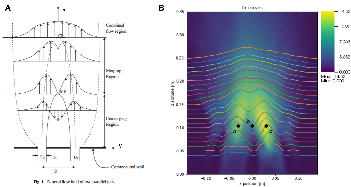
\includegraphics[width=14.7cm]{mixing_state_v4.pdf}}
    \slantedcaption{A. Definitions of three mixing states, taken from \cite{Durve2012Numericalinvestigationof}. B. TFI field on a 2D cross-section at $y$ = \SI{0.09}{\meter} and 1D profiles. Points a, b, and c are the reference points used for 1D sequential analysis.}
    \label{fig:mixing_state}
\end{figure}

\cite{Durve2012Numericalinvestigationof} also carried out a comparative study on several models for predicting the mean temperature field and temperature fluctuation field caused by mixing phenomena of the three jets \parencite{Durve2010Thermalstripingin}.
They performed a comparative study of root mean square temperature 1D profiles along the $x$ axis depending on the distance from the flow outlet,
i.e. the $z$ altitude direction in our study, Figure \ref{fig:durve2010}.
A comparison was done between one experimental ($\circ$) and three numerical simulation results (lines).
Each image in this figure shows the root mean square value of temperature measured/estimated for each normalized altitude $y/D_n$.
$y$ stands for the distance from the outlet of the jets, and $D_n$ is the diameter of the outlet.
The length along the horizontal direction ($x$ axis) is also normalized in the same way with the direction of altitude as $x/D_n$.
The root mean square values are also normalized by the temperature difference of the cold and hot jets ($\Delta T$).
The curves at each altitude do not match very well because of the difference of the compared model geometries.
For all experiment/simulation data, one can see the same transient behavior of the shape of curves, i.e.
the curves have two peaks at lower altitude, then these two peaks start to merge when the altitude increases, and finally the peaks merge completely.
Following different authors we choose to analyze the temperature in the medium using an index called the Temperature Fluctuation Intensity (TFI).
We use the definition of TFI as
\begin{align}\label{eq:4_1}
    TFI(\boldsymbol{r})=\sqrt{\frac{1}{N}\sum_{i=1}^{N}(T(i,\boldsymbol{r})-\bar{T}(\boldsymbol{r}))^2}, r=(x,y,z) \, ,
\end{align}
where
$\boldsymbol{r}$ is the spatial position vector,
$i$ is the time step number,
$N$ is the total number of time steps,
$T(i,\boldsymbol{r})$ is the temperature value at time step $i$ and position $\boldsymbol{r}$, and
$\bar{T}(\boldsymbol{r}) = \frac{1}{N}\sum_{i=1}^N T(i,\boldsymbol{r})$ is the average temperature at $\boldsymbol{r}$.
We process the PLAJEST Computational Fluid Dynamics (CFD) data to calculate the TFI index in order to compare the global behavior of the jets with these previous studies.
Figure \ref{fig:comp_durve2010} shows the same profile analysis with TFI values.
The normalized altitude $y/D_n$ and normalized horizontal position $x/D_n$ are adjusted to be the same as in \cite{Durve2012Numericalinvestigationof}'s figures.
TFI values are also normalized with $\Delta T =$ \num{43}\textdegree{}C, which is the temperature difference of the jets in the PLAJEST configuration.
Because of the difference of geometry and also of the medium (PLAJEST uses liquid sodium but the other studies use air or other liquids), the magnitude of the curves is not identical.
However, the shape of the curves follows the same way (i.e. two separated peaks $\rightarrow$ the peaks are merged gradually $\rightarrow$ the peaks are merged completely).

\begin{figure}[htbp]
    \centerline{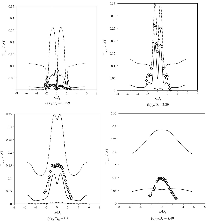
\includegraphics[width=12.0cm]{durve2010.pdf}}
    \slantedcaption{Comparison of normalized root mean square of temperature, taken from \cite{Durve2010Thermalstripingin}.}
    \label{fig:durve2010}
\end{figure}

Figure \ref{fig:mixing_state} B is the 2D cross-section at $y$ = \SI{0.09}{\meter} of the calculated 3D TFI field from the CFD results of PLAJEST.
There are three jets in the configuration of PLAJEST (the center position of the jets are $x$ = \SIlist{-0.070;0.0;0.070}{\meter}).
Between each jet, two zones with high TFI value arise by the interaction of these jet flows.
From this TFI field, it is found that for the shape of the TFI profile depending on the altitude, it seems to be possible to define three zones in a similar way as with the three zones for the mean flow field explained above.
First, the two high TFI zones arise around altitude $z$ = \SI{0.05}{\meter} and these two zones are completely separated.
Around altitude $z$ = \SI{0.09}{\meter} or lower altitude, the beginning of merging of the high TFI zones becomes clear (the lowest TFI value between two peeks starts to increase).
Here there would be some specific point that we call a merging point of the TFI zone.
The merging of these two zones is confirmed when the altitude becomes higher, and then around altitude $z$ = \SI{0.19}{\meter} these two zones are completely merged (the peak of the 1D TFI curve becomes a single one). We call this altitude a combining point of the TFI zone.

In the following section, we will carry out a more detailed analysis to verify the variations of the TFI profiles and the definition of these two points.
When we analyze the results of acoustic simulation, these two altitudes will be referred to and compared with the thermo-hydraulic state.
Thus, the main objectives of this chapter are to
see how an acoustic wave propagation fluctuation changes depending on the state of mixing flows.
In particular, we will try to find the relation between acoustic fluctuations and the changing points of the TFI 1D curves, which likely divide the TFI field into three zones (converging, merging and combined regions) as mentioned above.

\begin{figure}[htbp]
    \centerline{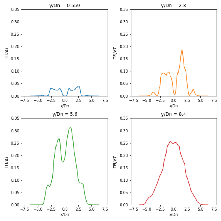
\includegraphics[width=12.0cm]{comp_durve2010.pdf}}
    \slantedcaption{Comparison of TFI 1D profiles calculated from the PLAJEST CFD results.}
    \label{fig:comp_durve2010}
\end{figure}

\section{Definition of the insonified volume}

The insonified volume is defined as a part of the PLAJEST volume displayed as a purple box in Figure \ref{fig:plajest_geo}.
In the geometry of PLAJEST, three sodium jets outflow from gaps with a \SI{20}{\milli\meter} width.
Multiple simulations are carried out with changing the $z$ coordinate of the extracted region from \SI{40}{\milli\meter} to \SI{340}{\milli\meter} above the outlet, with intervals of \SI{10}{\milli\meter}.
The temperature pattern just above the outlets is simple and stable, while it becomes more complex and unstable when the $z$ coordinate increases.
The magnitude of the fluctuations may be seen based on TFI visualization in Figure \ref{fig:mixing_state} B.
Multiple insonified volumes are then defined with the same volume size, same relative positions of the acoustic source and signal observing surfaces and with different altitudes.
In each insonified volume, a circular plane source is defined as in Figure \ref{fig:plajest_src}.
The color shows the maximum amplitudes of the emissions at each point normalized by the maximum amplitude at the center of the circle.
The plane source is composed of monopole point sources on a circular plane with a diameter of \SI{0.0254}{\meter} (i.e. 1 inch).
The intervals of each point sources are the same as the element size of the SPECFEM mesh.
Each source point emits a \SI{1}{\mega\hertz} Ricker wavelet (second derivative of a Gaussian) at the same time.
The maximum amplitude of each emission is multiplied by a Hamming window function depending on the distance from the center of the circle.
Figure \ref{fig:plajest_rec_def} shows the definitions of the observation surfaces of the acoustic signals.
On each plane, the receiving points where acoustic signals are recorded are placed with a \SI{0.0005}{\meter} pitch.
Figure \ref{fig:plajest_receiver_plane_geo} shows the positional relation between the insonified volume (central altitude $z$ = \SI{0.1}{\meter}) and the geometry of PLAJEST.
The numbers in meters show the distance from the source to each $y$-$z$ receiver plane.
The near field limit, called Io, is calculated to be \SI{67.17}{\milli\meter} using Equation \ref{eq:3_1}
and an average temperature of \num{333.167}\textdegree{}C (\num{606.317}\textdegree{}K), considering a transducer with a \num{1} inch diameter and \SI{1}{\mega\hertz} frequency.
In this virtual setup, only the first two observation surfaces are in the near field.
Thus, in the following analysis we mainly have acoustics virtual measurements in the far field.
In the PLAJEST coordinates the limit of the near field is $x$ = \SI{-0.061}{\meter}.

\begin{figure}[htbp]
    \centerline{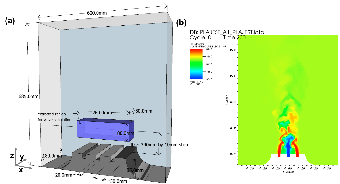
\includegraphics[width=16.0cm]{plajest_geo_v2.pdf}}
    \slantedcaption{(a) Geometry of the PLAJEST CFD simulation.  (b) Snapshot of the CFD result at time \SI{200.0}{\second}, $x$-$y$ cross-sectional plane at $y$ = \SI{0.09}{\meter}.
    Visualization for this image is done with VisIt, an open source visualization tool for massive scientific data \parencite{Childs2012VisItAnEnd}.}
    \label{fig:plajest_geo}
\end{figure}

\begin{figure}[htbp]
    \centerline{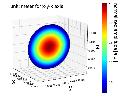
\includegraphics[width=13.0cm]{plajest_src.pdf}}
    \slantedcaption{The circular source plane used for the simulations.}
    \label{fig:plajest_src}
\end{figure}

\begin{figure}[htbp]
    \centerline{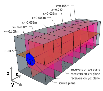
\includegraphics[width=13.0cm]{plajest_rec_def.pdf}}
    \slantedcaption{Positions of the plane source (blue) and receiver surfaces (orange and red). The $x$ position of the source plane is \SI{-0.128}{\meter}.}
    \label{fig:plajest_rec_def}
\end{figure}

\begin{figure}[htbp]
    \centerline{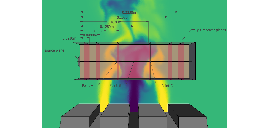
\includegraphics[width=18.0cm]{plajest_receiver_plane_geo_v3.pdf}}
    \slantedcaption{Relation of the positions in an insonified volume (central altitude $z$ = \SI{0.1}{\meter}) and the geometry of PLAJEST.
The points A, B and C are the positions of the reference points used for temporal analysis.}
    \label{fig:plajest_receiver_plane_geo}
\end{figure}

\section{Mesh generation and interpolation of the temperature field from Tetra4 elements to Hexa27 elements}

CEA/STMF used a numerical code for CFD calculations called TrioCFD (known as Trio\_U by 2015) for this PLAJEST numerical simulation, and LES was selected as the turbulence model.
Tetrahedral elements with 4 nodes were used for the TrioCFD calculations. The total number of elements was \num{5582706} and the characteristic mesh length was set to \SI{1.40}{\milli\meter}. We removed the first \SI{200}{\second} of their calculation from their result because that duration corresponds to the stabilization of the flow state.
Thus, \numrange{200}{210}\si{\second} with a time step of \SI{0.1}{\milli\second} is available as candidates for our wave simulation.
Three jets of sodium exist in this setup. Sodium with lower temperature (304.5\textdegree{}C) is emitted from the central jet, and with higher temperature (347.5\textdegree{}C) from the two outer jets. The average flow velocity is \SI{0.51}{\meter\per\second} for every jet (Figure \ref{fig:plajest_jaea} B).
The simulated temperature field at time = \SI{200.000}{\second} is shown in Figure \ref{fig:plajest_cea} (C). Their simulation results are in good agreement
with the experiment results obtained by JAEA in terms of normalized time-averaged temperature, normalized time-averaged temperature fluctuations, spectral power density and standard deviation of temperature values (Figure \ref{fig:plajest_cea} A, B and D).

For their calculation, a tetrahedral unstructured staggered mesh was used.
Temperature field values are defined at the center of each TrioCFD's tetrahedral mesh element, and flow velocity values are defined on the vertex nodes.
We thus had to transfer these values to our hexahedral mesh for SPECFEM3D.
To do so, we used interpolation onto each node of the SPECFEM3D hexahedral mesh using the simulation data management tool called MEDCoupling.
MEDCoupling is part of the pre-/post-processing platform SALOME (\url{http://www.salome-platform.org}) and is also available independently as a library.
Figure \ref{fig:temp_field_interpolation_processs} shows the temperature field data transfer and mesh generation steps as a pre-process for SPECFEM3D simulation.
Our hexahedral mesh for SPECFEM3D is built using the meshing software CUBIT developed by Sandia National Laboratories (USA).
Figure \ref{fig:interp_examp} shows some examples of this step. It is possible to select an arbitrary volume to be extracted from the entire geometry
and meshing is completed automatically, including the assignment of material characteristics and absorbing surface flags (the fluctuation of the temperature field may be defined later).
In this step, the region to be used for wave propagation simulation is specified in order to eliminate acoustically uninteresting parts from the PLAJEST geometry and thus reduce the required amount of computer memory, which is one of the limitations of wave simulations in large 3D models.
In order to speed-up this conversion process, we used the IOSS (IO Systems) library included in the finite-element analysis supporting software called SEACAS, also developed by Sandia National Laboratories.
After finishing preparation of mesh data, we carried out the temperature field transfer, i.e. interpolation of temperature values defined at the barycenter of each tetrahedral finite element to corner nodes of our hexahedral spectral elements.
The flow velocity data is not used for our simulation because we apply the frozen fluid hypothesis, as in \parencite{Massacret2012Simplifiedmodelingof}.
The conversion of the temperature field from TrioCFD tetrahedral mesh to SPECFEM3D nodes is done by using MEDCoupling.
Because the mesh-to-node transfer function does not support HEXA27 (second-order hexahedral finite elements), if the interpolation-target mesh is of HEXA27 type,
then HEXA27 first needs be split into eight parts of HEXA8 type (first-order hexahedral finite elements).

Determination of the element size to use in our simulations is done based on two conditions, which are the CFL condition (Equation \ref{eq:4_810}) and the number of
elements per one wave length:
\begin{align}\label{eq:4_810}
    C_p\frac{\Delta t}{\Delta x_{gll}} \leq \alpha \, ,
\end{align}
where $\Delta t$ is the time step and $\Delta x_{gll}$ is the minimum interval between two GLL grid points.
We selected the averaged Courant number $\alpha$ = \num{0.4} and the wave celerity $C_p$ = \SI{2416.268}{\meter\per\second} (in sodium with the lowest
temperature value \num{274.5} \textdegree{}C in the CFD simulation) for the calculation of the mesh size and time step duration.
In equation \ref{eq:4_810}, $\Delta x_{gll}$ is not the mesh size itself, it is the interval between GLL grid points inside the spectral elements.
This led us to use a mesh size $\Delta x$ = \SI{8.05d-4}{\meter} and a time step of \SI{2.3d-8}{\second}.
We will simulate a total of 5000 steps in order to have a sufficient total physical duration for the waves to travel through
the entire simulation domain. The mesh used in our simulations thus \num{3250000} spectral elements and a total number of GLL grid nodes of \num{215320764}.

\begin{figure}[htbp]
    \centerline{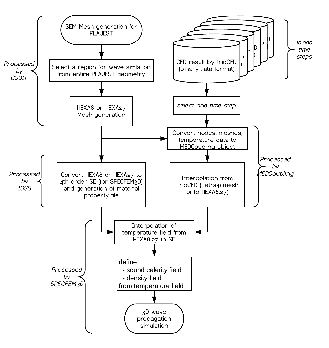
\includegraphics[width=18.0cm]{temp_field_interpolation_processs_v5.pdf}}
    \slantedcaption{Explanation of data processing for mesh generation and preparation of the heterogeneous medium to use for our acoustic calculations.}
    \label{fig:temp_field_interpolation_processs}
\end{figure}

\begin{figure}[htbp]
    \centerline{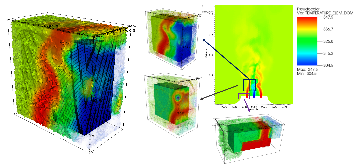
\includegraphics[width=17.0cm]{interp_examp_v2.pdf}}
    \slantedcaption{Examples of some interpolations of temperature fields from a tetrahedral mesh to a hexahedral mesh using the MEDCoupling pre/post-processing library.
The temperature field in the tetrahedral elements is indicated with transparent color on the interpolated field of the hexahedral mesh.
    The image on the left side is a close-up on one of these three examples.}
    \label{fig:interp_examp}
\end{figure}

\begin{figure}[htbp]
    \centerline{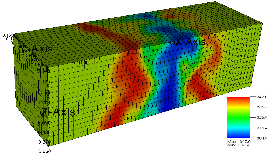
\includegraphics[width=16.0cm]{real_temp_field_sample.pdf}}
    \slantedcaption{One of the heterogeneous temperature fields used for our 3D wave propagation calculations. This field is taken from time step number 10,
and the central altitude of the calculation domain is \SI{0.1}{\meter} from the sodium outlet.
    One mesh contains 3,250,000 spectral elements and the total number of Gauss-Lobatto-Legendre grid points is 215,320,764.}
    \label{fig:real_temp_field_sample}
\end{figure}


\section{Results of acoustic wave propagation in a single temperature field}

In this part, we analyze the sensitivity of ultrasound to thermo-hydraulic changes.
The goal is to study how the ultrasonic beam is deflected or deformed by the temperature field.
In the following section, we will study the evolution of measurements as a function of time.

\begin{figure}[htbp]
    \centerline{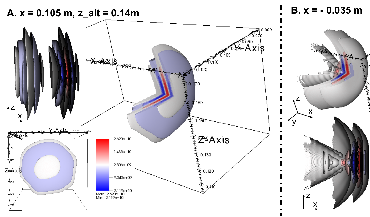
\includegraphics[width=16.0cm]{3dwavefronts_v3.pdf}}
    \slantedcaption{Visualization of the 3D wave front using contouring and clipping, at position $x$ = A) \SI{0.105}{\meter} and B) \SI{-0.035}{\meter} calculated at altitude $z$ = \SI{0.14}{\meter}, time = \SI{200.010}{\second} of PLAJEST with a heterogeneous medium temperature.}
    \label{fig:3dwavefronts}
\end{figure}

Figure \ref{fig:3dwavefronts} shows the visualized 3D wave fronts based on 3D contour visualization.
These waves are visualized from signals received in the $y$-$z$ receiver planes at time = \SI{200.010}{\second} in the CFD simulation and at altitude $z$ = \SI{0.14}{\meter}.
The left image is the wave front recorded at $x$ = \SI{0.105}{\meter} and the right image is recorded at $x$ = \SI{-0.035}{\meter}.
Color variations represent the signal amplitude values.
Blue is negative and red is positive.
In order to show the inside structure of the wave front, some contour surfaces are clipped off of its half or quarter volume.
The red part has higher pressure values and the blue part has lower ones.
The $y$ and $z$ axes correspond to the $y$ and $z$ axes of the PLAJEST geometry.
The $x$ axis indicates time.
For this 3D visualization, we used a VTK file (Visualization Toolkit: an open-source, freely available software system for 3D computer graphics, image processing, and visualization. \url{http://www.vtk.org}) that we displayed with the visualization software VisIt.
The visual information reveals that the wave fronts having passed through heterogeneous liquid sodium are deflected and deformed but that the amount of wave deformation is not so large.
The wave forms are different between waves passing from the end of the near field region to a far longer distance in the far field region (almost 4 $\times$ Io, where Io is the near field limit), and the wave front in the near field has the shape that is more complex than in the far field, as expected.
We will carry out a quantitative analysis of the amount of modification in the latter part of this chapter.
Figure \ref{fig:plajest_res1} shows part of the acoustic fields obtained from all of the simulations. Here an acoustic field refers to the maximum pressure values at each spatial point.
In figure \ref{fig:plajest_res1}, acoustic fields in the $x$-$y$, $y$-$z$ and $y$-$z$ plane (for $x$ = \SIlist{0.035; 0.105}{\meter}) are indicated for the simulations whose middle $z$ coordinate value are $z$ = \SIlist{0.04; 0.12; 0.24; 0.34}{\meter}. Additionally, the top row shows the results for the case with a homogeneous medium. In the homogeneous case, the temperature of medium was set to 333.167\textdegree{}C, which is the ambient temperature value of the CFD calculations.
From this figure, we find that the acoustic field at $z$ = \SI{0.040}{\meter}, which is close to the outlets, and the homogeneous case are quite similar.
This comes from the fact that the temperature boundary just above the outlets is almost orthogonal to the direction of wave propagation.
Also at z = \SI{0.340}{\meter}, the mixing of the hot and cold jets has matured enough and the magnitude of the temperature difference becomes small;
therefore, a wave is less affected by the heterogeneity at this altitude. However, at $z$ = \SIlist{0.120; 0.240}{\meter}, it can be seen that the acoustic fields
are bent by the heterogeneity of the field, and the reduction of maximum amplitude values with increasing propagation distance becomes greater.
This first qualitative description is then shown in Figure \ref{fig:plajest_res2} with 1D profiles of the acoustic field.

In Figure \ref{fig:plajest_res2}, values of the acoustic fields on the $z$ axis of each $y$-$z$ receiver planes are indicated.
The red lines represent the results of the homogeneous case and the blue lines represent all the results for the heterogeneous cases at each $z$ position of the simulation domain.
Amplitude values are normalized by the maximum amplitude (i.e. pressure) for all simulations.
How the maximum amplitude of pressure recorded in each $y$-$z$ receiver plane changes depending on the positional changes in the $z$ direction of the simulation domains is indicated in Figure \ref{fig:plajest_res3}.
At planes $x$ = \SIlist{-0.105; -0.080}{\meter}, i.e. near the plane source, maximum amplitudes take approximately constant values regardless of distance from the outlets.
In contrast, at the farthest and second farthest $y$-$z$ planes at $x$ = \SIlist{0.105; 0.080}{\meter}, it is found that the amplitude value of the simulation domain $z$ = \SI{0.120}{\meter} is approximately 10 \% smaller than the other values. At the same time the second peak may be found at $z$ = \SI{0.240}{\meter}.
It is considered that the effect of temperature heterogeneity becomes stronger under two conditions, which are:
\begin{itemize}
\item mixing of hot and cold flow are developed enough so that the shape of the temperature boundary is curved and not parallel to the emitted wave front,
\item the temperature difference remains large.
\end{itemize}
The altitude $z$ = \SI{0.120}{\meter} is the distance from the outlets where the temperature boundary starts to be changed while the temperature difference is still relatively still compared to the region above.
On the other hand, it seems that, at $z$ = \SI{0.240}{\meter}, the temperature difference is already small and even smaller than at $z$ = \SI{0.230}{\meter}.
This might be caused by the fact that the temperature boundary shape became a key factor for the whole effects rather than the temperature difference only.
As a result, we find that there is a certain relationship between the strength of effects of temperature heterogeneity on acoustic fields and the distance from the outlets of the sodium jets, i.e. the state of mixing flows. More precisely, the importance of these effects on maximum acoustic pressure can vary up to about 10 \% at a certain altitude.
Accordingly, we may assume that the magnitude of the temperature difference in a medium and the shape of the temperature boundary are the key factors
that govern the cumulated effects of medium heterogeneity on wave propagation.

A single time step was examined for this first study. In the next \autoref{sec:res_multi_time}, we will perform simulations with the same PLAJEST configuration for other time steps extracted from the CFD calculation in order to search for a relation between the strength of the medium heterogeneity and the variations of the ultrasonic signals.

\begin{figure}[htbp]
    \centerline{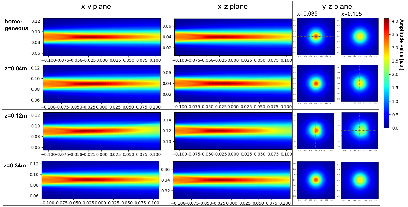
\includegraphics[width=16.0cm]{plajest_res1_v2.pdf}}
    \slantedcaption{Acoustic fields obtained from all the simulations.}
    \label{fig:plajest_res1}
\end{figure}

\begin{figure}[htbp]
    \centerline{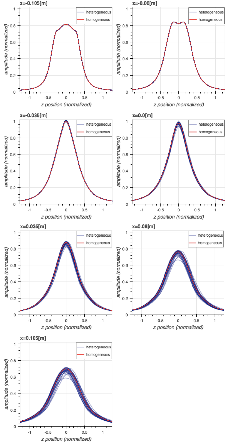
\includegraphics[width=12.0cm]{plajest_res2_v2.pdf}}
    \slantedcaption{Values of the acoustic fields on the $z$ axis at $y$ = 0 of each $y$-$z$ receiver plane.}
    \label{fig:plajest_res2}
\end{figure}

\begin{figure}[htbp]
    \centerline{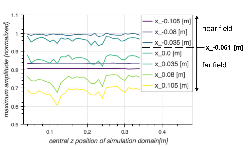
\includegraphics[width=14.0cm]{plajest_res3_v2.pdf}}
    \slantedcaption{The maximum amplitude of pressure recorded in each $y$-$z$ receiver plane changes depending on the positional change in the $z$ direction of the simulation domain.}
    \label{fig:plajest_res3}
\end{figure}

\section{Analysis of time-varying temperature fields of PLAJEST} \label{sec:res_multi_time}

\subsection{Selection of the CFD time steps to extract and analyze}

    The CFD calculation carried out by CEA STMF has approximately \SI{10}{\second} in total, from \SI{200.000}{\second} to \SI{210.197} with a \SI{0.001}{\second} interval.
The initial \SI{200}{\second} of the calculation was dedicated to ensuring stabilization of the flow and are thus excluded in our analysis.
    Because of the limitation of allocated computation time on the supercomputer that we use for this thesis, it was not possible to run the temperature field interpolation and wave propagation calculation processes for all of these CFD time steps.
    Instead, we had to extract several time steps of the temperature field with a wider interval from the CFD results.
    In order to select the time step interval to extract for our acoustic simulation, we used the power spectrum density curve \parencite{Angeli2015LargeEddySimulation} (Figure \ref{fig:PSD_angeli}, blue line). This curve indicates the temperature history at $x$ = \SI{-0.015}{\meter} (between the left and center jets), $y$ = \SI{0.09}{\meter} (middle point on the $y$ axis) and $z$ = \SI{0.1}{\meter}.
    From this curve, its peak is found lower than \SI{5}{\hertz} (around \SI{3}{\hertz}).
    Thus, to be sure to include the frequency of this \SI{5}{\hertz} temperature fluctuation, we extracted the temperature fields with a \SI{0.1}{\second} interval (i.e. \SI{10}{\hertz}).
    In a first approximation the peak was estimated to be around \SI{2}{\hertz}, and in that case we could expect to have 5 points per period to keep the peak at \SI{2}{\hertz}.
    This is the limit of Shannon's sampling criterion.

\begin{figure}[htbp]
    \centerline{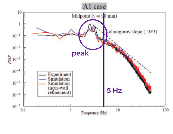
\includegraphics[width=12.0cm]{PSD_angeli.pdf}}
\vspace*{-1.6truecm}
    \slantedcaption{Normalized PSD curves of temperature history in the CFD calculation (blue line) at $x$ = \SI{-0.015}{\meter}, $y$ = \SI{0.09}{\meter} and $z$ = \SI{0.1}{\meter}, taken from \cite{Angeli2015LargeEddySimulation}. Normalized PSD curves are calculated by dividing the original PSD with the maximum PSD value.}
    \label{fig:PSD_angeli}
\end{figure}

    Figure \ref{fig:timestep_extraction} shows this relation between the CFD time steps and the extracted (sub-sampled) time steps for our acoustic simulations.
    Figure \ref{fig:psd_finer} shows the temperature histories and PSD curves of the original CFD results at three selected points, and Figure \ref{fig:psd_coarser} shows the same kind of curves but with only extracted time steps.
    These three points have the same $y$, $z$ position ($y$ = \SI{0.09}{\meter} and $z$ = \SI{0.1}{\meter}) and a different $x$ position ($x$ = \SIlist{-0.035;0.0;0.035}{\meter}).
    $x$ = \SIlist{-0.035;0.035}{\meter} are the positions between the two jets, and thus where the TFI will be higher than in the other areas.
    $x$ = \SI{0.0}{\meter} is in the middle of the central jet.
    These three points were selected in order to examine the thermo-hydraulics regime in three characteristic areas.
    The positional relation with the PLAJEST geometry is indicated by points A,B,C in Figure \ref{fig:plajest_receiver_plane_geo},
and the relation with the TFI is indicated by points a,b,c in Figure \ref{fig:mixing_state}.
    Using all the time steps of the CFD results, we calculated the PSD curves (Figure \ref{fig:psd_finer}).
    The peak of the PSD curve is confirmed at \SI{3}{\hertz}.
    Then PSD curves calculated from the coarser time step that we use in our acoustic simulations shows that the peak frequency at \SI{3}{\hertz} is conserved for the central point.
    From this comparison, we thus verify that the peak frequency of the temporal temperature fluctuation remains lower than the frequency limit that we selected for our acoustic simulation.
    Let us note however than in future work we plan to perform new calculations with a refined time step to describe these peaks more finely.

\begin{figure}[htbp]
    \centerline{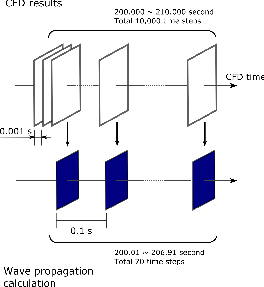
\includegraphics[width=11.0cm]{timestep_extraction.pdf}}
    \slantedcaption{Sampling intervals for the original CFD simulation and for our wave propagation simulation.}
    \label{fig:timestep_extraction}
\end{figure}

\begin{figure}[htbp]
    \centerline{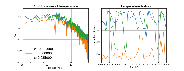
\includegraphics[width=20.0cm]{psd_finer_v2.pdf}}
    \slantedcaption{A. PSD curves and B. temperature histories of the CFD results at three different $x$ positions ($y$ = \SI{0.09}{\meter}; $z$ = \SI{0.1}{\meter}), with a 10 Hz sampling.}
    \label{fig:psd_finer}
\end{figure}

\begin{figure}[htbp]
    \centerline{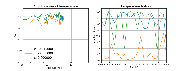
\includegraphics[width=20.0cm]{psd_coarser_v2.pdf}}
    \slantedcaption{A. PSD curves and B. temperature histories of the extracted time steps at three different $x$ positions, with a 10 Hz sampling.}
    \label{fig:psd_coarser}
\end{figure}

\subsection{Treatment of the massive amount of calculations and management of the results}

    In this study, all of simulations were performed on two of the largest supercomputers in Europe: CURIE (CEA TGCC) and OCCIGEN (CINES), both part of GENCI (Grand \'Equipement National de Calcul Intensif).
    The computation domain was divided into 256 parts, and parallelized calculations were carried out.
    The average duration for an acoustic simulation is about 26 minutes, excluding mesh generation and the interpolation processes of the temperature fields, which are done once and for all.
    The duration of the interpolation of a temperature field from a TrioCFD result to SPECFEM3D is approximately 20 hours using a single CPU for one acoustic simulation altitude of one time step.
    We carried out 70 time steps of interpolation of the 3D temperature field, for 22 difference altitudes, resulting in a total of 1540 acoustic simulations to perform.
As a result, the total time needed for a complete simulation of wave propagation over \SI{7}{\second} of the variable thermo-hydraulic regime is approximately equal to 687 hours, i.e. 29 days.
    Because of the huge number of calculations, the result data cannot be conserved as a 3D volume data because of the limitation of allocated storage on supercomputers.
    Instead of storing all results in 3D, we first selected the 2D planes in which we will analyze the acoustic signals (Figure \ref{fig:plajest_rec_def}).
    We then defined time windows for each $y$-$z$ plane to cut the received signals depending on the arrival time of the wave front.
    These time-windowed signals were then gathered as a single, huge HDF5 binary file.
    The HDF5 (Hierarchical Data Format) format is a standard and widely-sued binary file format that has been developed to manage extremely large and complex data collections.
    By using it, one can access the results faster than with other standard file formats such as e.g. ASCII, json, csv, pickle (Python-friendly binary data format) etc.

\subsection{Computing TFI data for comparison with acoustic simulation results}

    As introduced in Equation \ref{eq:4_1}, we resort to an index called Temperature Fluctuation Intensity (TFI), as used in \cite{Angeli2015LargeEddySimulation}.
    Because of the very large numbers of total time steps and also the huge number of mesh nodes included in the CFD calculation results,
the standard way to calculate the TFI value based on this equation is not very efficient.
    To calculate that TFI, we thus selected and implemented another, more advanced algorithm: the online algorithm, which we will briefly describe in this section.
    Figure \ref{fig:tfi3d} shows the calculated TFI field in 3D, and Figure {\ref{fig:tfi_with_field}} is the cross-section at $y$ = \SI{0.09}{\meter}.
We find that there are two areas where the TFI value becomes high between the sodium jets at altitude $z$ = \SIrange{0.08}{0.16}{\meter}.
    It should also be noted that the TFI field is not symmetric with respect to the $x$ center.

    The online algorithm calculates some field value from serial data sequentially and based on a single step \parencite{Knuth1997TheArtof}.
    This algorithm can be required for serial data for which each step needs a large amount of computer memory and/or when the number of serial data
is so large that it is very expensive to perform an entire loop of calculations more than twice.
    We thus applied this algorithm to compute the TFI, i.e. the standard deviation of the temperature value at a given point,
    because computing a standard deviation implies several loop over the whole time steps, first to calculate the mean temperature,
and second to calculate the difference between a temporal value and the mean value.
    The PLAJEST CFD data comprise 10,000 time steps of 3D volume data with 2,039,769 mesh elements.
    One entire loop calculation for this data takes about 10 hours.
    By applying the online algorithm for the calculation of the TFI, we only need to do this long loop calculation once.

\begin{figure}[htbp]
    \centerline{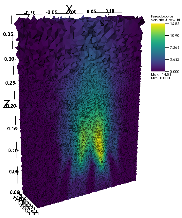
\includegraphics[width=10.0cm]{tfi3d_v3.pdf}}
    \slantedcaption{Visualized 3D TFI field.}
    \label{fig:tfi3d}
\end{figure}

    \begin{figure}[htbp]
        \centerline{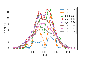
\includegraphics[width=12.0cm]{tfi_1d_v2.pdf}}
        \slantedcaption{TFI values on the $x$ axis and at $y$ = \SI{0.09}{\meter} at several altitudes.}
        \label{fig:tfi_1d}
    \end{figure}

    The definition of standard deviation of temperature at a given position $\boldsymbol{r}$ is
    \begin{align}\label{eq:4_2}
        \sigma^2 (\boldsymbol{r}) = \frac{1}{N}\sum_{i=1}^{N} (T(\boldsymbol{r},i) - \bar{T}(\boldsymbol{r}))^2 \, ,
    \end{align}
    where $N$ is the total number of time steps and $\bar{T}(\boldsymbol{r})=\frac{1}{N}\sum_{i=1}^{N}T(\boldsymbol{r},i)$ is the average temperature at position $\boldsymbol{r}$.
    In the online algorithm, the averaged value $\bar{T}(\boldsymbol{r},n)$ and the term $\sum_{i=1}^{n} (T(\boldsymbol{r},i) - \bar{T}(\boldsymbol{r}))^2 = M_{\boldsymbol{r},n}$
    are sequentially updated for each time step during the entire loop calculation.
    For each time step at $n$,
    \begin{align}\label{eq:4_3}
        \bar{T}_{\boldsymbol{r},n} = \bar{T}_{\boldsymbol{r},n-1} + \frac{T_{\boldsymbol{r},n} - \bar{T}_{\boldsymbol{r},n-1}}{n}
    \end{align}
    \begin{align}\label{eq:4_4}
       M_{\boldsymbol{r},n}=M_{\boldsymbol{r},n-1}+ (T_{\boldsymbol{r},n} - \bar{T}_{\boldsymbol{r},n-1})(T_{\boldsymbol{r},n} - \bar{T}_{\boldsymbol{r},n})
    \end{align}
    The standard deviation calculation is then finalized as
    \begin{align}\label{eq:4_5}
        \sigma_{\boldsymbol{r}}=\sqrt{\frac{M_{\boldsymbol{r},N}}{N}} \,.
    \end{align}

   \begin{figure}[htbp]
        \centerline{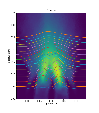
\includegraphics[width=12.0cm]{tfi_with_field.pdf}}
        \slantedcaption{TFI curves corresponding to the 2D TFI field. The left side shows the $z$ altitude where those lines are extracted.}
        \label{fig:tfi_with_field}
    \end{figure}

    Figure \ref{fig:tfi_1d} shows the TFI values on the $x$ axis of $y$ = \SI{0.09}{\meter} at several altitudes (i.e. $z$ positions), and Figure \ref{fig:mixing_state} B represents these TFI curves drawn in the case of the 2D TFI field.
    The maximum TFI value is found at around altitude $z$ = \SI{0.13}{\meter}. The change of shape of the curves depending on the distance from the exit of the jets seems to match with the result of \cite{Durve2010Thermalstripingin},
    i.e. the curves at low altitude have two TFI peaks, and then these peaks gradually merge when the $z$ altitude increases.
    We will further analyze this effect in the next sections of this chapter.

\subsection{Calculating the "Cumulated TFI" (CTFI) value}

    The TFI calculated above is the index that evaluates the intensity of the fluctuation at one spatial point,
while acoustic wave propagation will be affected not only by one position but by the whole state along its propagation path.
    Thus, in order to find the appropriate thermo-hydraulic index for comparison in the case of a propagating wave, we define a new index, which we call the cumulated TFI (CTFI).
    The CTFI is the value that indicates the amount of TFI that the acoustic wave experiences along the central axis.
    We define the CTFI at the position $x_p$ in the propagation direction by
    \begin{align}\label{eq:4_6}
        {I_c}(x_p,z_{alt},R) = \int_{x_{s}}^{x_{p}} \int_0^R \int_0^{2\pi} I(r,\theta,z_{alt}) w(r) d\theta dr dx \,
    \end{align}
    where
    $I_c$ is the CTFI value,
    $I(x,r,\theta)$ is the TFI value at $x,r,\theta$,
    $x_s$ is the x coordinate of acoustic source,
    $z_{alt}$ is the altitude (along the $z$ axis) of the center of the acoustic source plane,
    $R$ is the distance from the central axis, and
    $w(r)$ is a weight function to make TFI values near the central axis have more effect and TFIs far from the central axis less effect.
One can define several versions of the CTFI, for instance:
\begin{enumerate}
\item CTFI in 1D (integrated on the central $x$ axis), with $w(r) = 1$ and $R = $ one mesh element size,
\item CTFI in 3D A (integrated in a domain where the acoustic beam passes), with $w(r) = 1$ and $R = $ the radius of the acoustic source, i.e. 1.27 cm,
\item CTFI in 3D B (integrated in a cylindrical volume where the acoustic beam passes, with a weighting function $w(r) = 0.54 + 0.46 cos{\pi \frac{r}{R}}$ and $R = $ the radius of the acoustic source, i.e. 1.27 cm.
\end{enumerate}
Using a larger $w(r)$ allows us to take into account the whole ultrasonic beam.
A more complex function will be needed to take into account the beam divergence.
In this thesis, we only use the first definition of the CTFI, i.e. the CTFI in 1D, as a first analysis.
The other possible choices may be examined in future work.

Figure \ref{fig:ctfi_1d} indicates the CTFI curves on the $x$ axis at $y$ = \SI{0.09}{\meter} and at several $z$ altitudes.
The left image shows the CTFI depending on the $x$ position, i.e. the propagation distance. The source plane is positioned at $x$ = \SI{-0.128}{\meter}.
Each line represents the $z$ altitude at which the curves are extracted.
The magnitude of the CTFI becomes largest around the altitude $z$ = \SI{0.13}{\meter}.
The curves for a lower $z$ altitude exhibit a two-step increment, as there are two peaks of TFI as we saw in the last section.
At a position higher than \SI{0.16}{\meter}, this two-step increment is no longer seen.
The right image represents the CTFI values versus altitude $z$.
Each line represents the $x$ position, i.e. propagation distance (the acoustic source is placed at $x$ = \SI{-0.128}{\meter}).
The farther the $x$ position becomes, the larger the magnitude of the CTFI becomes as well.
We find that the peak of the CTFI positions is around \SIrange{0.13}{0.15}{\meter}.
For the $x$ position = \SI{0.00}{\meter} just after the first (left side of) the high TFI zone and the middle of the central jet,
the CTFI peak is slightly shifted to a higher $z$ altitude.
This is caused by the slight difference is the shape and position of the high TFI zones, as one can see in Figure \ref{fig:ctfi_with_field}.
Figure \ref{fig:ctfi_2nd} shows the second derivatives of the CTFI curves.
The inflection points are found around $z$ = \SI{0.09}{\meter} and \SI{0.19}{\meter}.
These points are the same altitudes as what we defined as the merging point and combining point of the standard TFI.
Thus, from this result, we find that we can define the merging and combing points of the TFI as the inflection points of the second derivatives of the CTFI curve.

In the following part of this chapter, we will study the acoustic fluctuation state based on these merging and combining points.

\begin{figure}[htbp]
    \centerline{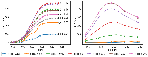
\includegraphics[width=17.5cm]{ctfi_1d_v4.pdf}}
    \slantedcaption{CTFI curves on the $x$ axis at $y$ = \SI{0.09}{\meter} and at several $z$ altitudes.}
    \label{fig:ctfi_1d}
\end{figure}

\begin{figure}[htbp]
    \centerline{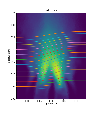
\includegraphics[width=12.0cm]{ctfi_with_field.pdf}}
    \slantedcaption{CTFI curves corresponding to the 2D TFI field.
On the left side once can see the altitude $z$ at which these lines are extracted.}
    \label{fig:ctfi_with_field}
\end{figure}

\begin{figure}[htbp]
    \centerline{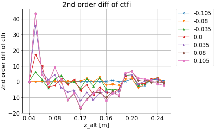
\includegraphics[width=12.0cm]{cfti_2nd_v2.pdf}}
    \slantedcaption{Second derivatives of the CTFI 1D profiles. Each line indicates the $x$ position.}
    \label{fig:ctfi_2nd}
\end{figure}

\section{Comparison with acoustic simulation results}

\subsection{Fluctuation of acoustic signals}

    First, we investigate the transition of the deviated wave front at the farthest $y$-$z$ receiving plane (i.e. $x$ = \SI{0.105}{\meter} and at a distance from the source of \SI{0.233}{\meter}).
    Figure \ref{fig:move_impact_points} shows the impact points, i.e. the position where the pressure value becomes maximum in the $y$-$z$ receiving plane.
In order to show temporal changes of the positions of the impact points more clearly, the positions of the impact points are linked by arrows in temporal order,
and digits are added to indicate the order in which the position of the impact point changes.
    Histograms for the $y$ and $z$ axis directions are also placed, showing the mean and standard deviation values.
    We confirm that the standard deviation is the largest at altitude $z$ = \SI{0.13}{\meter} (number 3 of \ref{fig:move_impact_points}).
    This is in good agreement with the peak $z$ position of the CTFI in Figure \ref{fig:ctfi_1d}.
    At lower altitude $z$ = \SIlist{0.04;0.09}{\meter}, the distribution of the impact points exhibits directivity, i.e. the standard deviation for the $y$-axis direction is larger than for the $z$-axis direction.
    This result illustrates the fact that the 3D temperature fluctuation pattern before maturing of the mixing state has directivity.
Namely, approximating the fluctuation of the acoustic celerity field using an isotropic Gaussian random process may not be very accurate for the regions where the flow is still strong.
    From this result, we can confirm the observation by \cite{Iooss2002Numericalsimulationof} of the non-applicability of an isotropic Gaussian random field for this region in a quantitative way.
Part of this directivity effect may be caused by the geometry of PLAJEST, because the cross-sections on the $y$ axis of PLAJEST always have the same shapes.
    However, in the real geometry of a SFR, for instance ASTRID, which has outlet tubes with a larger diameter (\SI{0.15}{\meter}) than in the PLAJEST experiment (\SI{0.02}{\meter}), the same effect may occur depending on the directions of the acoustic beam towards the sodium jets, even if the shape of the jets is cylindrical.

\begin{figure}[htbp]
    \centerline{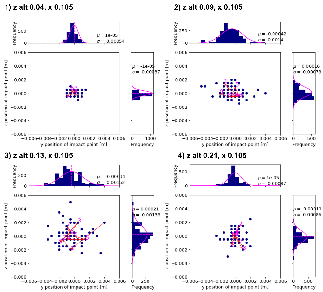
\includegraphics[width=16.0cm]{move_impact_points_v2.pdf}}
    \slantedcaption{Movement of acoustic impact points (i.e. the position at which acoustic pressure becomes the largest) in the $y$-$z$ receiving plane at $x$ = \SI{0.105}{\meter}, and histograms for the $y$ and $z$ directions. Movements of only the seven initial time steps are indicated with red arrows and with digits in magenta.}
    \label{fig:move_impact_points}
\end{figure}

    We also carried on an acoustic fluctuation analysis.
    Figure \ref{fig:acoust_sig_1d_fluc} shows the history of maximum amplitude and the time at which the maximum amplitude is received, as well as the normalized PSD curves.
    Maximum amplitude values are taken from the envelope of each received signal.
    The figures on the left column are the history of maximum amplitude value (in blue), receiving times (in red) and temperature (in green).
    The figures on the right column are the PSD curves of the three values, in the same colors as the history curves.
    The results received at four different altitudes, at $x$ = \SI{0.105}{\meter}, $y$ = \SI{0.09}{\meter} and $z$ = \SIlist{0.04;0.09;0.14;0.21}{\meter} are shown.
    At the lowest altitude ($z$ = \SI{0.04}{\meter}), the magnitude of fluctuation of the signal is the smallest among the four positions.
    At altitude $z$ = \SIlist{0.09;0.14}{\meter}, the magnitude of fluctuation becomes larger, and then
    at a higher altitude ($z$ = \SI{0.21}{\meter}), the magnitude of fluctuation again becomes smaller than at $z$ = \SI{0.09}{\meter} and \SI{0.14}{\meter}.
    Compared with the CFTI values, the shape of fluctuation magnitude seems to match with the CTFI curve.
    From the PSD at altitude $z$ = \SI{0.04}{\meter}, the peak of both amplitude and receiving time is before \SI{1}{\hertz}.
    When the altitude becomes higher, only the peak of receiving time becomes \SI{3}{\hertz}, as the peak frequency of temperature fluctuation in Figure \ref{fig:psd_finer}.
    However, in the PSD curve of maximum amplitude, the peak seems to be found around \SI{1.8}{\hertz}, but it is weak (i.e. there are other small peaks).
    At this $x$ position, temperature fluctuation is almost zero.
    Thus it is not possible to compare the temperature fluctuation and the fluctuation of acoustic signals.
    In order to see if the fluctuation state of temperature has an effect on the acoustic fluctuation at $x$ = \SI{0.105}{\meter},
    the same history curves and PSD are indicated for different $x$ positions in Figure \ref{fig:ac_1d_comp_x}.
    At $x$ = \SI{0.0}{\meter}, maximum amplitude, receiving time and temperature have no peaks on their PSD curves.
    At $x$ = \SI{0.035}{\meter}, a peak at \SI{3}{\hertz} is found for the PSD of temperature as well as for the PSD of receiving time, but maximum amplitude has no peak.
    It should be noted that the magnitude of the temperature fluctuation is the largest among other $x$ positions.
    At $x$ = \SI{0.105}{\meter}, temperature has no fluctuation while the peak at \SI{3}{\hertz} of the PSD of receiving time remains.
    Maximum amplitude still has only a weak peak around \SI{1.8}{\hertz}.
    These results show that the fluctuation of time of flight at one receiving position may result not only from the fluctuation state of temperature at the receiving point only,
    but also from other locations around the propagation path, where the magnitude of temperature fluctuation is strong
and that may thus have a dominant effect on the acoustic signal observed later in the propagation.
    In summary, the spectral analysis of the amplitude fluctuations does not make it possible to highlight a dominant frequency. The spectrum in particular is strongly noisy.
    On the other hand, the spectrum of time of flight fluctuations, especially when they are of great amplitude (in the merging region),
reveals a dominant frequency that is consistent with the frequency of temperature fluctuations in the mixing zone.
    These preliminary results could be refined by a frequency analysis performed with a smaller time step.

\begin{figure}[htbp]
    \centerline{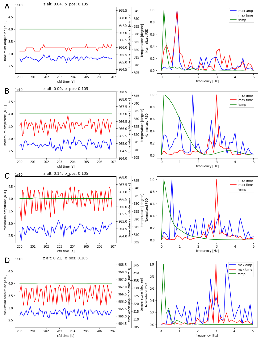
\includegraphics[width=17.0cm]{acoust_sic_1d_fluc_v2.pdf}}
    \slantedcaption{History of maximum amplitude (in blue), arrival time (in red) and temperature (in green), and the normalized PSD curves,
    for four different altitudes, at $x$ = \SI{0.105}{\meter}, $y$ = \SI{0.09}{\meter} and $z$ = \SIlist{0.04;0.09;0.14;0.21}{\meter}.}
    \label{fig:acoust_sig_1d_fluc}
\end{figure}

\begin{figure}[htbp]
    \centerline{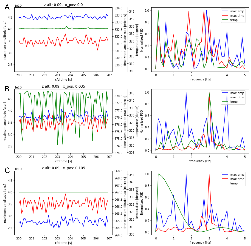
\includegraphics[width=17.0cm]{ac_1d_comp_x.pdf}}
    \slantedcaption{History of maximum amplitude (in blue), arrival time (in red) and temperature (in green), and the normalized PSD curves,
    for three different $x$ position, at $x$ = \SIlist{0.0;0.035;0.105}{\meter}, $y$ = \SI{0.09}{\meter} and $z$ = \SI{0.09}{\meter}.}
    \label{fig:ac_1d_comp_x}
\end{figure}

\subsection{Standard deviation analysis}

    In order to get additional information that will help to interpret the fluctuation of the acoustic signals,
    we also carried out a standard deviation and mean value analysis for the whole of $z$ altitudes based on the following four acoustic quantities:
    \begin{itemize}
        \item maximum amplitude at the impact point and at the center of the $y$-$z$ plane,
        \item amount of deviation $r$,
        \item angle at the impact point $\theta$,
        \item receiving time of the maximum amplitude at the center of the $y$-$z$ plane.
    \end{itemize}
    Figure \ref{fig:impactpoint} shows the definition of the impact point, of $r$, and of $\theta$.

    \begin{figure}[htbp]
        \centerline{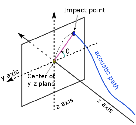
\includegraphics[width=9.0cm]{impactpoint_v4.pdf}}
        \slantedcaption{Definition of the impact point, of the amount of deviation $r$, and of the deviation angle $\theta$.}
        \label{fig:impactpoint}
    \end{figure}

    Figure \ref{fig:std_amps} shows the standard deviation and mean values of maximum amplitude values recorded at the center and at the impact point of each $y$-$z$ plane.
    Part 1 shows the standard deviation and mean value of maximum amplitudes at the center of the $y$-$z$ planes for each $z$ altitude.
    Part 2 shows the same values but recorded at the impact points.
    Each line is the mean value, and the error bar is the standard deviation at each position.
    The scale of values on the vertical axis is the same for the mean values, and the length of the error bars as well.
    We note that the mean values of maximum amplitude of each $x$ position are not very different between the different $z$ altitudes.
    In Part 3, only the mean values of maximum amplitude are plotted (solid line: $y$-$z$ center, dashed line: impact point).
At the $x$ positions far from the acoustic source ($x$ = \SIlist{0.035;0.08;0.105}{\meter}), differences of means between the $y$-$z$ center and the impact point are observed.
    This comes from the fact that the impact points always records the maximum amplitude of an acoustic wave front, thus the mean value may be larger than at the $y$-$z$ center.
    $x$ = \SI{-0.08}{\meter} is in the near-field (or Fresnel) zone, thus the difference between the maximum pressure value and the value of pressure on the axis (i.e. pressure at the center of the $y$-$z$ plane) is large.
    Part 4 shows standard deviations divided by mean values at each $z$ altitude.
    At altitudes in the range $z$ = \SIrange{0.10}{0.15}{\meter}, the standard deviation at each $x$ position becomes larger than at other altitudes.
    By applying a moving average triangular window with a window length of 8, we obtain Part 5.
    The scatter plots are the standard/mean values before smoothing, and the lines represent smoothed curves.
    The curves have similar peak positions as the CTFI curves of Figure \ref{fig:ctfi_1d} and also exhibit the same position of their inflection points when computing
their second derivatives (Part 6).
    Thus, the inflection points of standard/mean curves of maximum amplitudes occur at the altitudes of the merging point and combining point of the TFI values.

\begin{figure}[htbp]
    \centerline{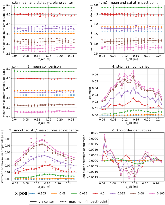
\includegraphics[width=17.0cm]{std_amps_v3.pdf}}
    \slantedcaption{
    1: Comparison of maximum magnitude at the center of each $y$-$z$ receiving plane.
    2: Comparison of maximum magnitude at the acoustic impact point, i.e. the location where the pressure value becomes maximum in each $y$-$z$ plane.
    3: Comparison of the mean value of maximum amplitudes. The solid lines are the values at the $y$-$z$ plane center, and the dashed lines are the values at the impact points.
    4: Comparison of standard deviation values divided by the mean value for each $z$ altitude.
    5: Standard/mean curves smoothed by a moving average window.
    6: Second derivatives of smoothed standard/mean curves.}
    \label{fig:std_amps}
\end{figure}

    Figure \ref{fig:std_r} is the analysis of the deviation length $r$.
    Part 1 indicates mean curves with solid lines and Part 2 shows standard deviation curves.
    The peak positions are also similar with the maximum amplitude curves, i.e. the peaks of the $x$ = \SIlist{0.035;0.08;0.105}{\meter} curves occur around altitude $z$ = \SIrange{0.13}{0.14}{\meter}.
    The curves in Part 3 are smoothed mean curves, and Part 4 shows the second derivatives of these means.
    Part 5 and Part 6 are smoothed standard deviations and their derivatives.
    Using Part 4 and Part 6, we can also find the inflection points for the mean and standard deviation curves at the merging point and combining point of the TFI.

\begin{figure}[htbp]
    \centerline{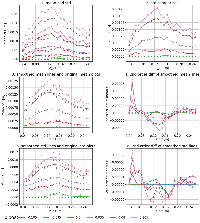
\includegraphics[width=18.0cm]{std_r_v3.pdf}}
    \slantedcaption{
    1: Comparison of the mean and standard deviation of deviation length $r$. The solid line is the mean value and the dashed line is the mean plus the standard deviation.
    2: Comparison of standard deviation only.
    3: Mean curves smoothed with a moving average window.
    4: Second derivatives of the smoothed mean lines.
    5: Standard deviation curves smoothed with a moving average window.
    6: Second derivatives of the smoothed standard deviation lines.}
    \label{fig:std_r}
\end{figure}

    Figure \ref{fig:std_theta} shows the mean and standard deviations of $theta$ as defined in Figure \ref{fig:impactpoint}.
    The solid lines are the mean angles and the dashed lines are the mean plus standard deviations and mean minus standard deviations.
    At altitudes lower than \SI{0.15}{\meter}, the mean angle is shifted in the first quadrant.
    Thus, in this region, the deflection of acoustic beams has directivity.
    At altitudes higher than \SI{0.15}{\meter}, the mean angle is still shifted but from the deviation length $r$, which has smaller values at these high altitudes as seen in Figure \ref{fig:std_r}, and there is no more directivity of deflection.
    From these results, we find that the directivity of the deflection effect on acoustic propagation exists at lower altitude, where the sodium flow is still strong and mixing between jets has not matured yet.
    Because of this, the isotropic Gaussian random field representation is not applicable for this area because isotropic Gaussian fields have no directivity effects on wave propagation.
    This altitude \SI{0.15} was the position at which CTFI curves for $x$ = \SI{0.105}{\meter} became maximum.

\begin{figure}[htbp]
    \centerline{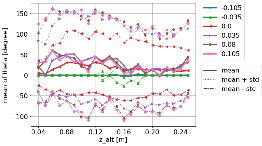
\includegraphics[width=13.0cm]{std_theta_v2.pdf}}
    \slantedcaption{Comparison of standard deviation and mean values of deviation angle $\theta$.}
    \label{fig:std_theta}
\end{figure}

    Finally, let us analyze the simulation results based on the fluctuation of times of flight, i.e. the receiving time of the signal.
    Figure \ref{fig:def_tof} shows the definition of the initial wave and of the time of flight.
    The position where simulation time is taken equal to zero is the center of the Ricker wavelet (second derivative of a Gaussian).
    We define the receiving time (the time of flight) as the peak position of the signal envelope.
    Let us recall that there are several classical (and different) ways to measure time of flight in practice.
Using the signal envelope is one of them, and it is useful in particular when the beginning of the signal can be masked by the noise \parencite{Chaki2007CombinationofLongitudinal}.
    The figures in \ref{fig:std_tof} show the change of mean and standard deviation of times of flight at each $z$ altitude of each $x$ position.
In the figure for $x$ = \SI{-0.105}{\meter}, almost no fluctuation of time of flight is found, except at altitudes in the range \SIrange{0.18}{0.22}{\meter}.
    As one can see in the TFI field of Figure \ref{fig:tfi_with_field}, even if the $x$ position is before the first jet,
a fluctuation of the medium still occurs because the fluctuating field diffuses when the flows go higher.
    At $x$ = \SI{-0.08}{\meter}, this character of the mixing jet can be confirmed from the fact that the altitudes at which time of flight values fluctuate become wider and located a little lower than $x$ = \SI{-0.105}{\meter}.
    Then, at $x$ = \SI{-0.035}{\meter} the standard deviation curve becomes wider, with its peak position located at about $z$ = \SI{0.16}{\meter},
while the mean curve has its peak at lower altitude, at about \SI{0.08}{\meter}.
    This peak position of the mean time of flight is caused by the difference of mean temperature from the acoustic source to the receiving point between different altitudes.

    Figure \ref{fig:mean_profile} Parts 1 and 2 show the transition of mean temperature from the acoustic source to the receiving point.
    Parts 3 and 4 show the mean sound speed profiles.
    From Part 3 it is clearly seen that around $x$ = \SI{-0.035}{\meter} the mean sound speed becomes low, especially when the altitude is low.
This is the reason why the mean time of flight curve at $x$ = \SI{-0.035}{\meter} has its peak at low altitude.
On the other hand, around $x$ = \SI{0.035}{\meter}, the mean sound speed becomes higher when the altitude is high, and this causes smaller values of the mean time of flight (Figure \ref{fig:std_tof}).
    Figure \ref{fig:std_tof2} shows the second derivatives calculated from mean values (left) and from standard deviations (right) of the times of flight.
    A moving average window is applied to both the mean and standard derivative curves to obtain these second derivatives in an accurate way.
    As the other derivative curves presented previously, i.e. for maximum amplitude and for $r$, these curves also exhibit two inflection points.
It is worth noticing that these two points are still in agreement with the possible merging point and combining point defined from the thermo-hydraulic regime.

\begin{figure}[htbp]
    \centerline{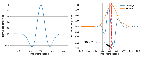
\includegraphics[width=15.0cm]{def_init_rec.pdf}}
    \slantedcaption{Definition of the source time function (left) and of time of flight (right).}
    \label{fig:def_tof}
\end{figure}

\begin{figure}[htbp]
    \centerline{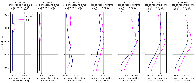
\includegraphics[width=18.0cm]{std_tof_v2.pdf}}
    \slantedcaption{Comparison of standard deviation (magenta) and mean (blue) values of receiving time.
The range of the horizontal axis of each figure is the same for both the mean and the standard deviation.}
    \label{fig:std_tof}
\end{figure}

\begin{figure}[htbp]
    \centerline{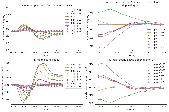
\includegraphics[width=17.0cm]{cmeantemp_1d_v2.pdf}}
    \slantedcaption{
1: Mean temperatures from source to receiver.
2: Mean temperatures from source to receiver, depending on $z$.
3: Mean sound speed.
4: Mean sound speed, depending on $z$.}
    \label{fig:mean_profile}
\end{figure}

\begin{figure}[htbp]
    \centerline{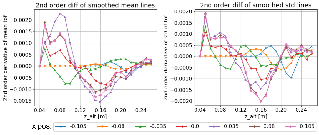
\includegraphics[width=17.0cm]{std_tof2.pdf}}
    \slantedcaption{Second derivatives of the mean (left) and standard deviation (right) of time of flight.}
    \label{fig:std_tof2}
\end{figure}

\section{Conclusions of this chapter}

    In this chapter, we studied the effect of a realistic heterogeneous temperature field on wave propagation in four dimensions (i.e., three spatial dimensions + time).
    We first simulated wave propagation at a (single) given instant of an existing CFD simulation,
changing the altitude of the insonified zone in order to find the amount of effect of the sodium state in the PLAJEST experiment on wave propagation.
    We exhibited certain altitude ranges at which a strong effect may occur on acoustic wave propagation.
    We then carried out the same acoustic simulation but for multiple CFD time steps in order to investigate the relation between the altitude of the insonified zone
and the thermal-hydraulic state.
    A standard deviation and mean analysis was done in order to study the possible amount of fluctuation of the acoustic signals.
    From an analysis of temperature fluctuation, we defined two altitudes at which the state of temperature fluctuation changes:
one is the merging point, where the two high TFI zones between each of three jets start to merge,
and the other is the combining point of the TFI, where the merging of the TFI zones is completed.
    These altitude can be detected as inflection points of the second derivative of the CTFI curves.

    From the 1D comparison between the fluctuation of temperature, of maximum amplitude and of time of flight, we showed
    that the fluctuation of time of flight at one receiving position may be affected not only from the fluctuation state of temperature at the receiving point only,
    but also from the temperature fluctuation state at other locations along the propagation path, which may have a dominant effect on the acoustic signal when the magnitude of temperature fluctuation is strong at these locations.
    We also showed that the frequency of temperature fluctuations in the merging zone could be deduced from the frequency of fluctuations of acoustic measurements, at least in the case of times of flight.
    As a result of our standard deviation and mean analysis, we found that at the low altitude where the mixing of flows is not enough matured, the temperature heterogeneity may cause directive fluctuation of acoustic propagation.
    This means that the application of an isotropic Gaussian random field may not take into account the directive response of fluctuation of acoustic signals.
This comes from the fact that the fluctuating values generated by an isotropic Gaussian random field always have a normal distribution and no directivity.
    We also found that the second derivatives of the mean and standard deviation of acoustic fluctuations (maximum amplitude, amount of deviation $r$, and time of flight) may have inflection points at altitudes close to those at which we defined the merging and combining points.

